In this section, we show the empirical performance of our algorithm GDSDA-SVM on the benchmark dataset Office. Specifically, we provide two different settings: single source and multi-source transfer scenarios for GDSDA-SVM.

\textbf{Dataset:}
There are 3 subsets in Office datasets, Webcam (795 examples), Amazon (2817 examples) and DSLR (498 examples), sharing 31 classes. In our experiments, we use DSLR and Webcam as the source domain and Amazon as the target domain.
We use the features extracted from Alexnet \cite{KrizhevskyNIPS12} FC7 as the input features for both source and target domain. The source models are trained with multi-layer perception (MLP) on the whole source dataset. 

\subsection{Single Source for Office datasets}
In this experiment, we compare our algorithm under the setting where there is just one source model. Specifically, we perform two groups of experiments using Amazon dataset as the target domain and DSLR and Webcam datasets as the source domains respectively. As we mentioned, there are significantly fewer labeled examples than unlabeled ones in real SDA applications.
Therefore, in each group of experiment, we just use 1 labeled example per class with 3 different sizes of unlabeled example (10, 15 and 20 per class).
%we set the size of the labeled example to be 1 per class, and the size of the unlabeled example to be 10, 15 and 20 per class respectively.

To demonstrate the effectiveness of GDSDA-SVM, we show the performance of GDSDA using brute force to search the imitation parameter $\lambda$ in the range $[0,0.1,...,1]$ with different temperature $T$ as the baselines. Meanwhile, we show the performance of the source model on the target task, denoted as "Source" and the performance of a target model (using LIBLINEAR\cite{fan2008liblinear}) trained with only labeled examples in the target domain denoted as "No transfer"\footnote{We fail to achieve a better performance using semi-supervised learning method \cite{delalleau2005efficient} on the target data as the no transfer baseline (may due to the size of the initial labeled examples).}. To avoid the randomness, we perform each experiment 10 times and report the average result. For GDSDA-SVM, we use temperature $T=20$ for all experiments in this part. The experimental results are shown in Figure \ref{fig:single1}. 
%$\lambda$ on the X-axis of the figures denotes the imitation parameter for the hard label and the corresponding imitation parameter for the soft label is set to $1-\lambda$.

From the results of brutal force search, it is clear that the value of imitation parameter can greatly affect the performance of the target model.
Also, we can see that, when we only use the unlabeled data for distillation, i.e. $\lambda = 0$, as we expected, GDSDA can still slightly outperform the source model. This means GDSDA can effectively transfer the knowledge between different domains under the unsupervised scenario. As we increase the value of imitation parameter, i.e. introducing the hard labels from the target domain, the performance of GDSDA can be further improved. As we mentioned before, even though our "fake label" strategy would introduce extra noise, the noise can be limited by setting the proper value to imitation parameter and the target model can still get improved performance compared to the baselines.

Moreover, we can see that GDSDA-SVM can achieve the competitive results compared to baselines using brutal force search in D$\rightarrow$A experiments. In W$\rightarrow$A experiments, it achieves the best performances on all 3 different unlabeled sizes. This indicates that we can effectively (about 6 times faster than brutal force search) obtain a good target model with GDSDA-SVM.
%\newpage
%\subsubsection{From DSLR to Amazon}
\begin{figure}[t]
\centering
\begin{tabular}{cccc}
\subfloat[D $\rightarrow$ A, 10 unlabeled ]{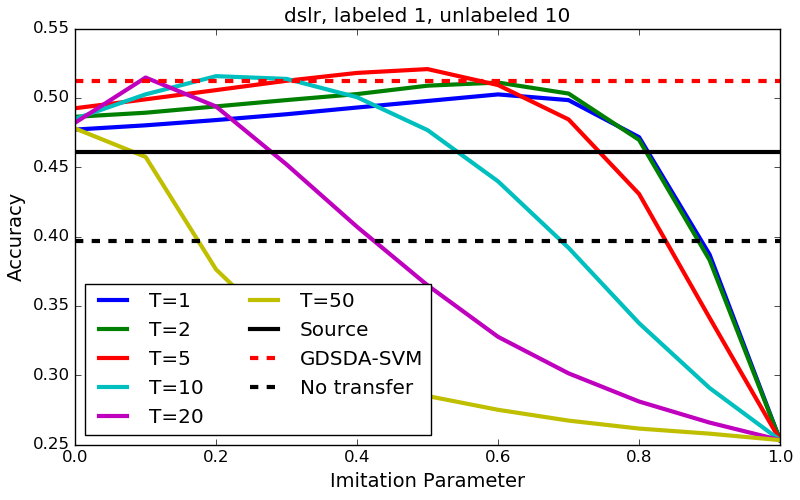
\includegraphics[width=0.3\textwidth]{figure/dslrtoamazonlabeled1unlabeled10.png}}&
\subfloat[D $\rightarrow$ A, 15 unlabeled ]{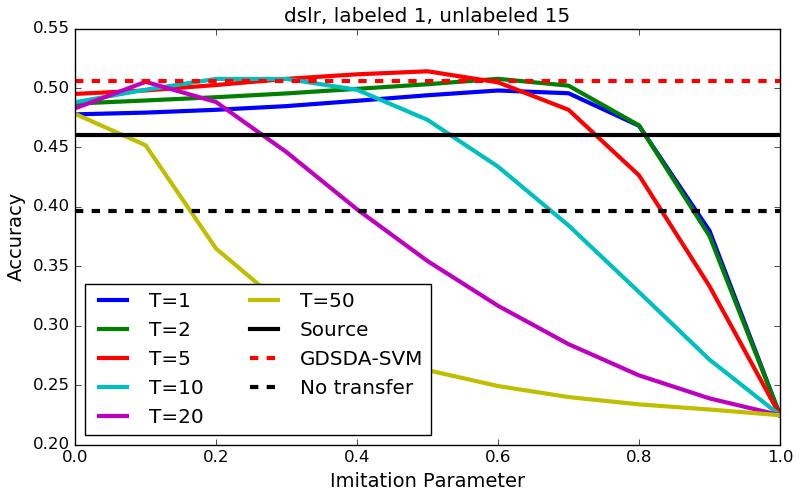
\includegraphics[width=0.3\textwidth]{figure/dslrtoamazonlabeled1unlabeled15.png}}&
\subfloat[D $\rightarrow$ A, 20 unlabeled ]{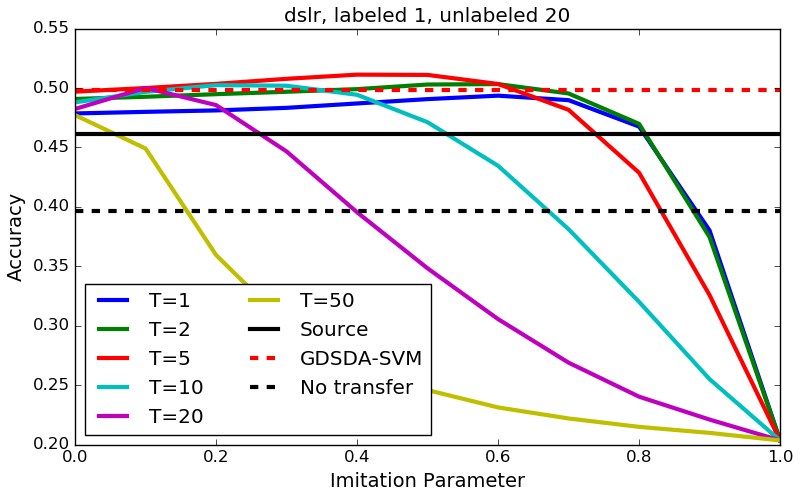
\includegraphics[width=0.3\textwidth]{figure/dslrtoamazonlabeled1unlabeled20.png}}\\
\subfloat[W $\rightarrow$ A, 10 unlabeled ]{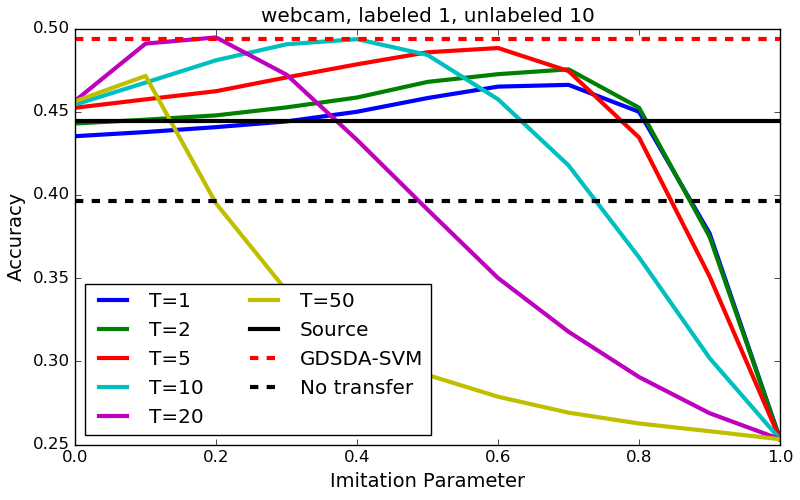
\includegraphics[width=0.3\textwidth]{figure/webcamtoamazonlabeled1unlabeled10.png}}&
\subfloat[W $\rightarrow$ A, 15 unlabeled ]{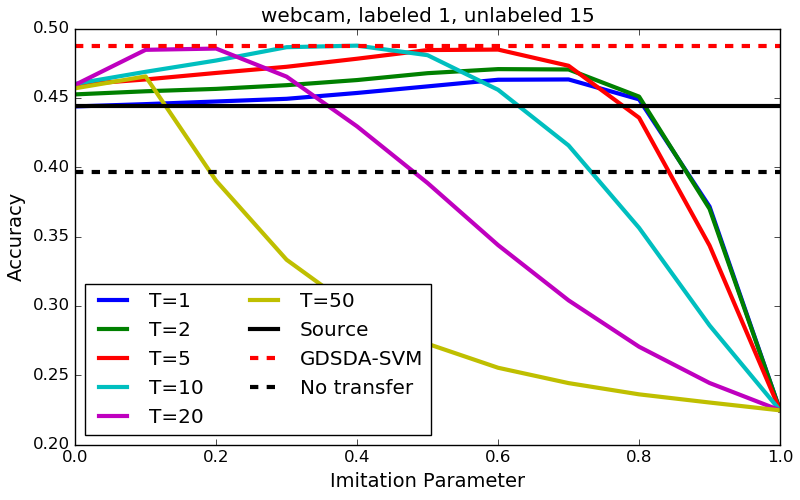
\includegraphics[width=0.3\textwidth]{figure/webcamtoamazonlabeled1unlabeled15.png}}&
\subfloat[W $\rightarrow$ A, 20 unlabeled ]{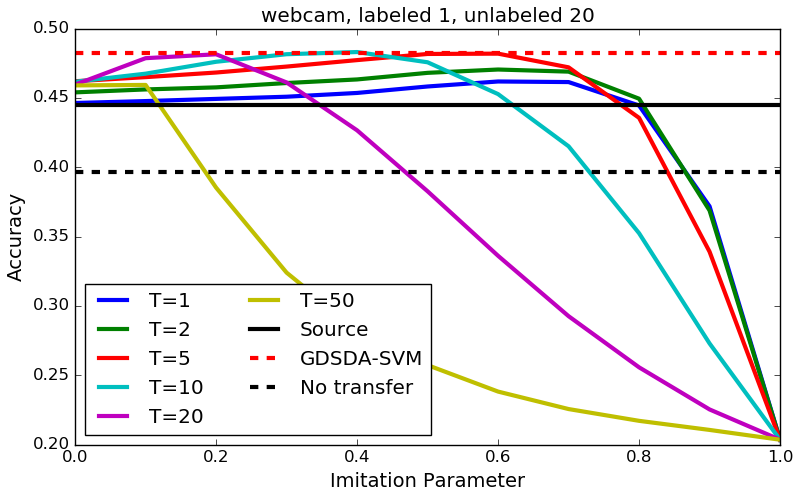
\includegraphics[width=0.3\textwidth]{figure/webcamtoamazonlabeled1unlabeled20.png}}\\
\end{tabular}
\caption{Experiment results on DSLR$\rightarrow$Amazon and Webcam$\rightarrow$Amazon when there are just one labeled examples per class. The results of DSLR$\rightarrow$Amazon and Webcam$\rightarrow$Amazon are shown in figure (a)-(c) and (d)-(e) respectively. GDSDA-SVM is trained with temperature $T=20$. $\lambda$ on the X-axis denotes the imitation parameter of the hard label and the corresponding imitation parameter of the soft label is set to $1-\lambda$.
}\label{fig:single1}
\end{figure}
\subsection{Multi-Source for Office datasets}
\begin{figure}
	\centering
	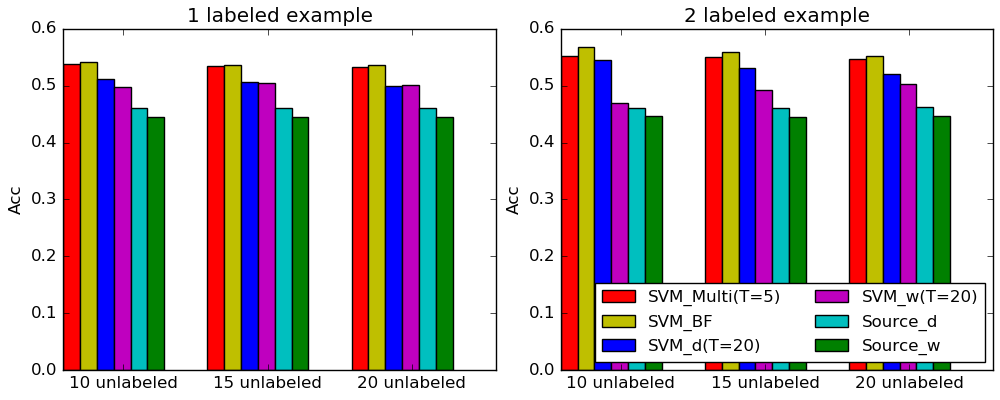
\includegraphics[scale=.4]{figure/cmp.png}
	\caption{D+W$\rightarrow$A, Multi-source results comparison.}\label{fig:multi}
\end{figure}
In this experiment, we show the performance of GDSDA-SVM under the multi-source SDA scenario.
Specifically, we train the target model for the Amazon dataset and adapt the knowledge from the rest of two source domains, Webcam and DSLR.
We use the similar settings as our single source experiment and perform 2 groups of experiments using 1 labeled and 2 labeled examples per class respectively. We use temperature $T=5$ and the results of multi-source GDSDA-SVM are denoted as SVM\_Multi. Here we use two single source GDSDA-SVMs (SVM\_w and SVM\_d trained with Webcam and DSLR respectively) as the baselines. We also show the best performance of the brutal force search model (SVM\_BF). We search temperature in range $T=[1,2,5,10,20,50]$ and each imitation parameter in range $[0,0.1,...,1]$. The experiment results are shown in Figure \ref{fig:multi}.

From the results, we can see that, given 2 source domains, SVM\_Multi can still leverage the knowledge effectively and outperform any single source model trained with GDSDA. This shows that the imitation parameter estimated by our method can effectively balance the importance of each source to achieve improved performance. SVM\_Multi performs slightly worse than the best result found by brutal force search in some experiments. However, considering their time complexity (GDSDA-SVM is around 30 times faster than brutal force search), SVM\_Multi still has its advantage in real applications.




